
		
		\subsection{IU1 Pantalla de Iniciar sesi\'on}

\subsubsection{Objetivo}
	Verificar si el usuario que est\'a intentando entrar al sistema sea el correcto y ya se encuentra registrado en el sistema de mensajer\'ia.

\subsubsection{Dise\~no}
	Esta pantalla aparece al ingresar al sistema de mensajer\'ia. 

	\begin{figure}[htbp!]
		\centering
			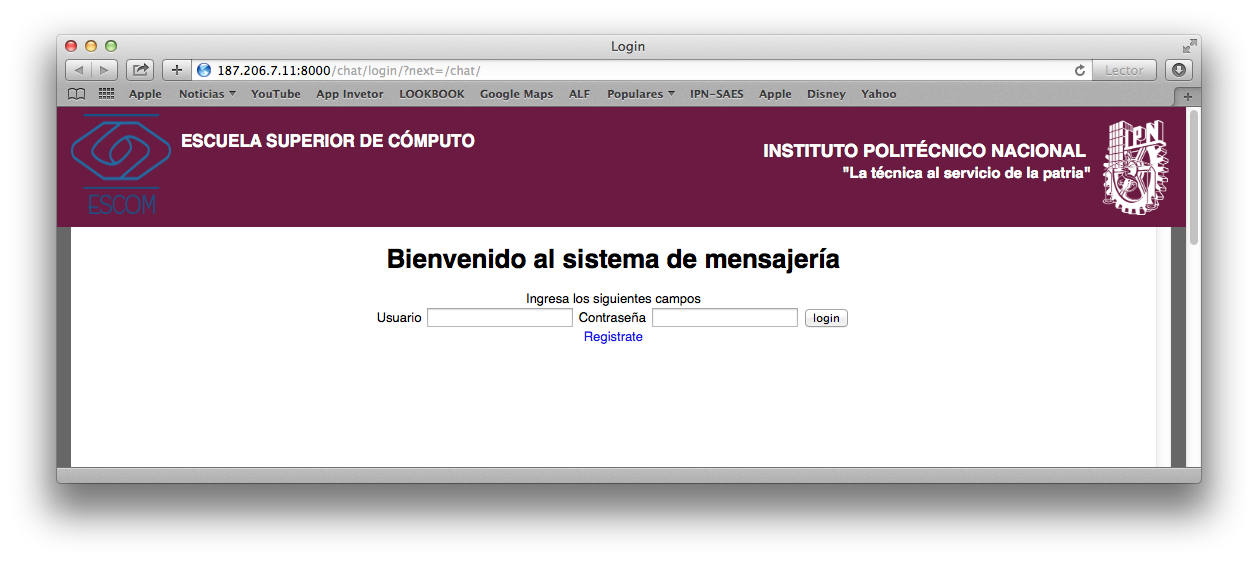
\includegraphics[width=0.9\textwidth]{images/Modulo1/Login}
		\caption{Pantalla de inicio de sesi\'on.}
	\end{figure}

\subsubsection{Salidas}
Ninguna


\subsubsection{Entradas}
\begin{Citemize}

\item Usuario 
\item Contrase\~na
\end{Citemize}

\subsubsection{Comandos}
\begin{itemize}
	\item \IUbutton{Login}: Verifica que el usuario se encuentre registrado en la base de datos y de ser as\'i verifica que la contrase\~na corresponda al usuario. 
	\item \IUbutton{Reg\'istrate}: Muestra el formulario que el usuario necesita llenar para poder registrarse en el sistema.
\end{itemize}

\subsubsection{Mensajes}
	\begin{Citemize}
		\item {\bf MSG1} Forbidden.	\end{Citemize}
		
	\pagebreak		%%%%%%%%%%%%%%%%%%%%%%%%%%%%%%%%%%%%%%%%%%%%%%%%%%
		
		\subsection{IU2 Pantalla de Registro de usuario}

\subsubsection{Objetivo}
	Registrar a un usuario con el objetivo de obtener sus datos principales y que \'este posteriormente pueda hacer uso del sistema de mensajer\'ia.

\subsubsection{Dise\~no}
	Esta pantalla aparece al dar clic en el bot\'on \IUbutton{Registrarte} que se encuentra al final de la pantalla de inicio.

	\begin{figure}[htbp!]
		\centering
			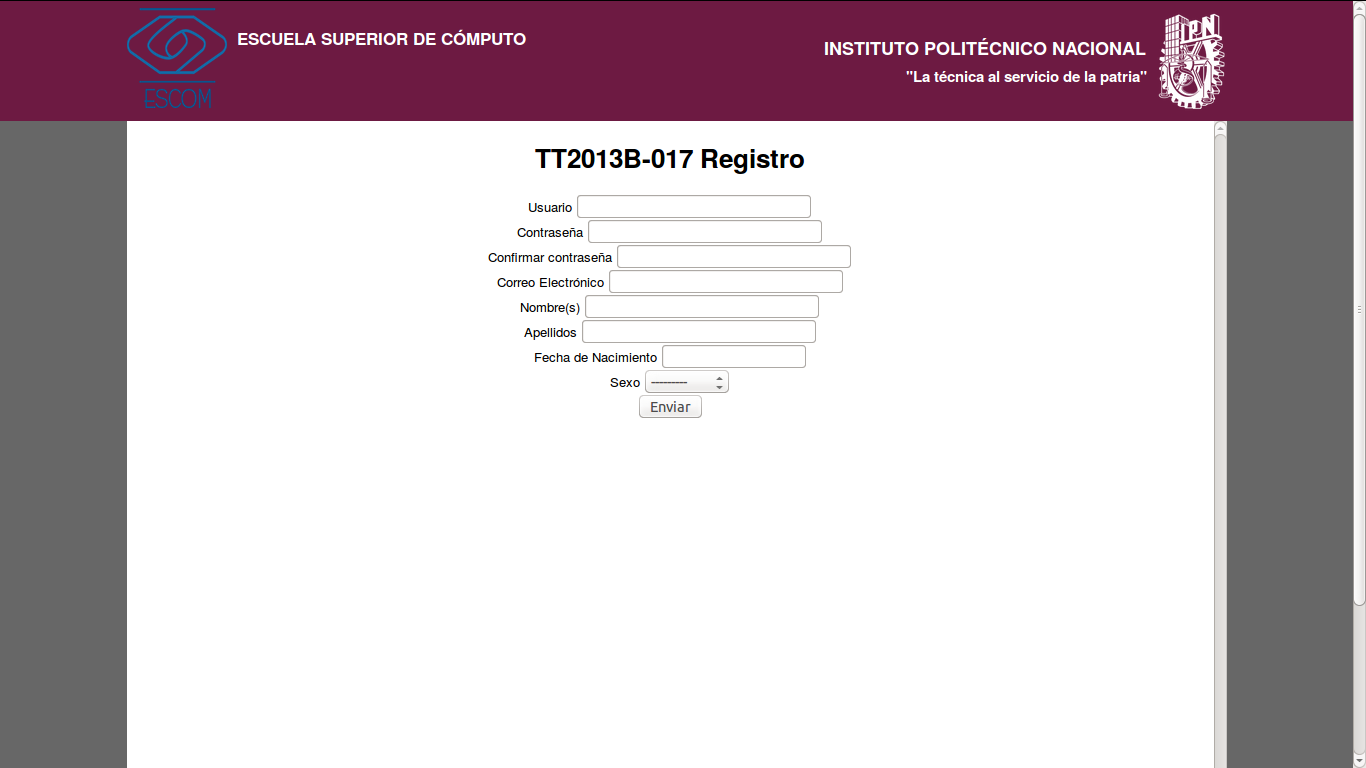
\includegraphics[width=0.8\textwidth]{images/Modulo1/Registro}
		\caption{Pantalla de registro de usuario.}
	\end{figure}

\subsubsection{Salidas}
	\begin{Citemize}
		\item {\bf MSG1} Ha sido registrado correctamente.	
	\end{Citemize}
	


\subsubsection{Entradas}
\begin{Citemize}

\item Usuario 
\item Contrase\~na
\item Correo electr\'onico 
\item Nombre
\item Apellidos
\item Fecha de nacimiento
\item Sexo
\end{Citemize}

\subsubsection{Comandos}
\begin{itemize}
	\item \IUbutton{Enviar}: Ingresa los datos del usuario a la base de datos, si estos fueron ingresados correctamente muestra el mensaje de registro exitoso. \end{itemize}
	\begin{figure}[htbp!]
		\centering
			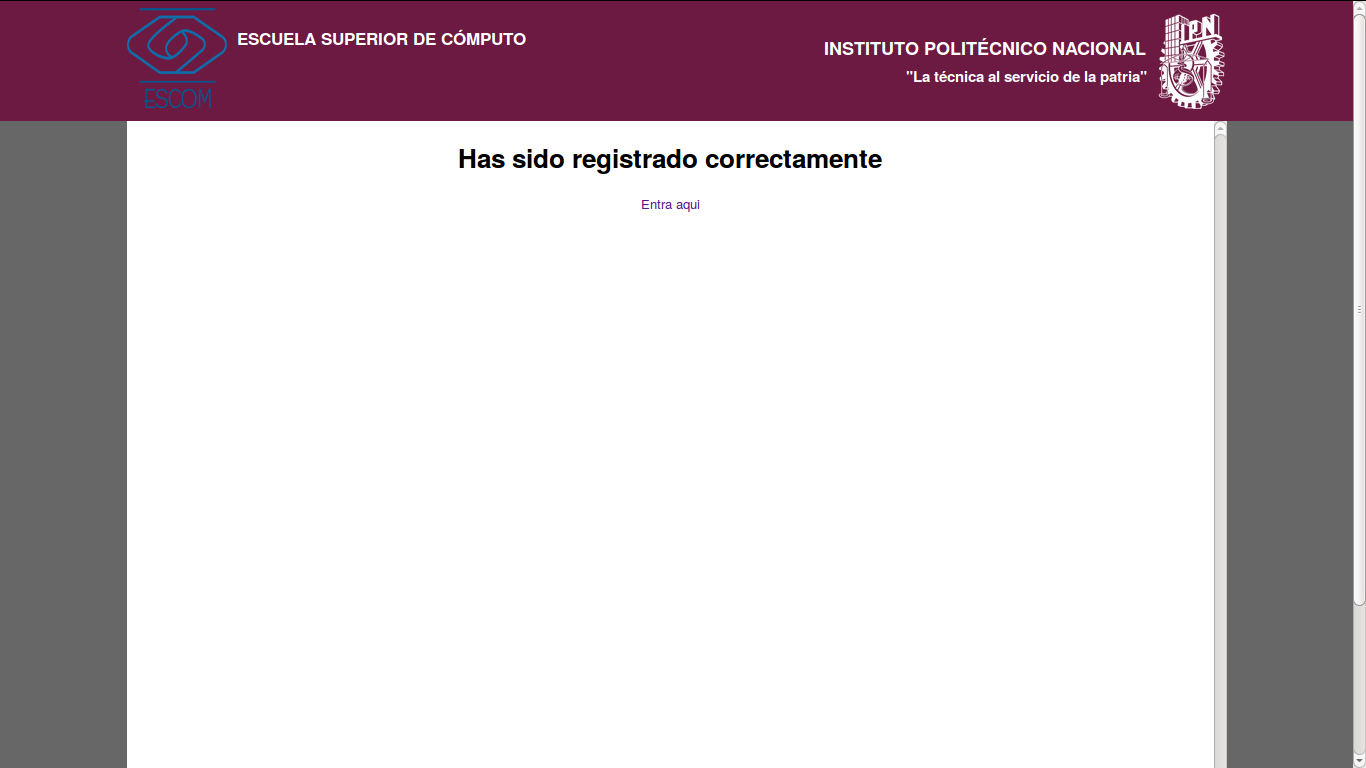
\includegraphics[width=0.9\textwidth]{images/Modulo1/SalidaRegistro}
		\caption{Mensaje de registro exitoso.}
	\end{figure}
\subsubsection{Mensajes}
	\begin{Citemize}
		\item {\bf MSG2} This field is required.	\end{Citemize}
		
			\pagebreak%%%%%%%%%%%%%%%%%%%%%%%%%%%%%%%%%%%%%%%%%%%%%%%%%%
	\subsection{IU3 Pantalla de Conversaciones}

\subsubsection{Objetivo}
	El objetivo de esta pantalla es que el usuario pueda visualizar las conversaciones que tiene, es decir, los contactos que forman parte de su lista.

\subsubsection{Dise\~no}
	Esta pantalla aparece al iniciar sesi\'on correctamente.

	\begin{figure}[htbp!]
		\centering
			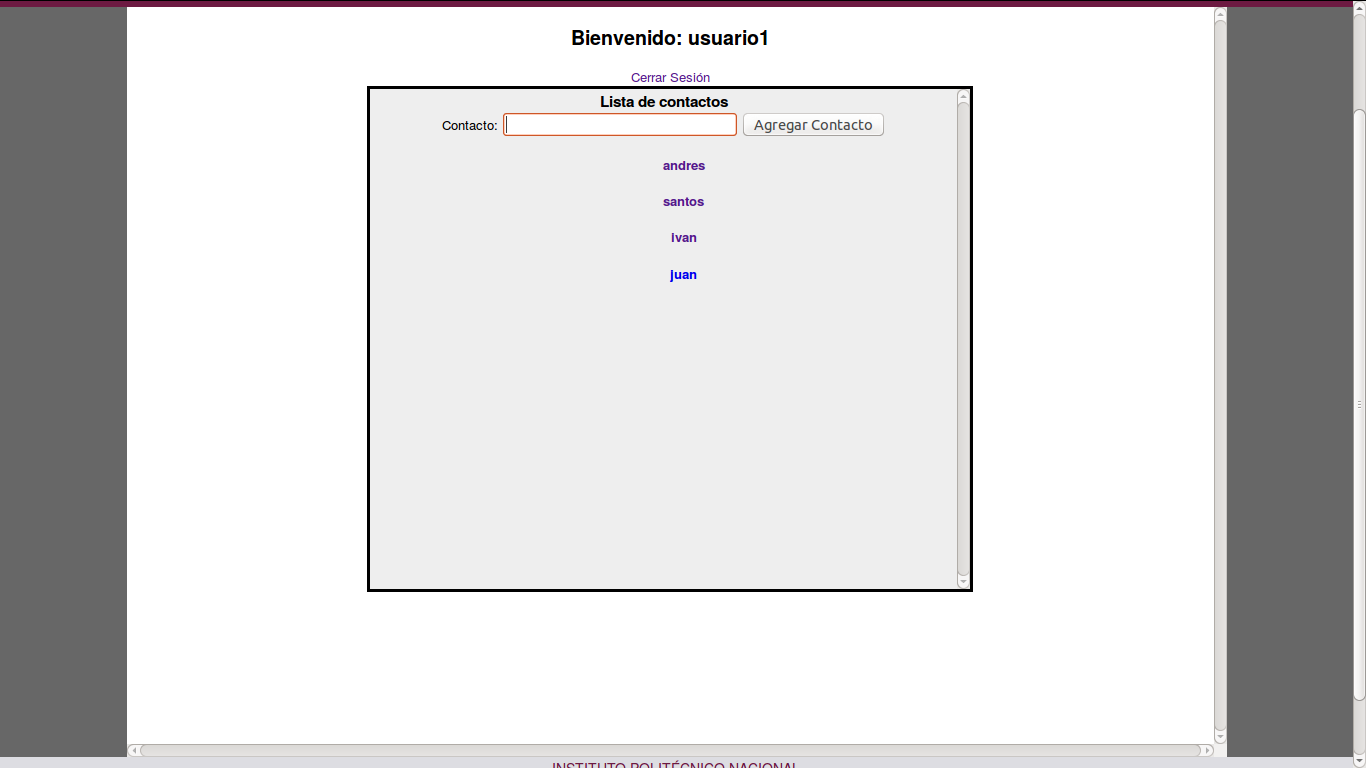
\includegraphics[width=0.9\textwidth]{images/Modulo1/Conversaciones}
		\caption{Pantalla de conversaciones}
	\end{figure}

\subsubsection{Salidas}
Lista de Contactos (conversaciones)


\subsubsection{Entradas}
\begin{Citemize}


\item Contacto
\end{Citemize}
\subsubsection{Comandos}
\begin{itemize}
			\item \IUbutton{"Contacto"}: Muestra la conversaci\'on del Contacto seleccionado y permite el intercambio de mensajes.
			\item \IUbutton{Cerrar sesi\'on}: Termina la sesi\'on y regresa a la p\'agina de inicio.
	\end{itemize}

\subsubsection{Mensajes}
Ninguno

		
	\pagebreak		%%%%%%%%%%%%%%%%%%%%%%%%%%%%%%%%%%%%%%%%%%%%%%%%%%
	
	
	
		
		\subsection{IU4 Pantalla del Sistema de Mensajer\'ia}

\subsubsection{Objetivo}
	El objetivo de esta pantalla es que el usuario pueda enviar y recibir mensajes de otros usuarios conectados.

\subsubsection{Dise\~no}
	Esta pantalla aparece al elegir el Contacto con el cual se desea intercambiar mensajes o analizar conversaciones pasadas.

	\begin{figure}[htbp!]
		\centering
			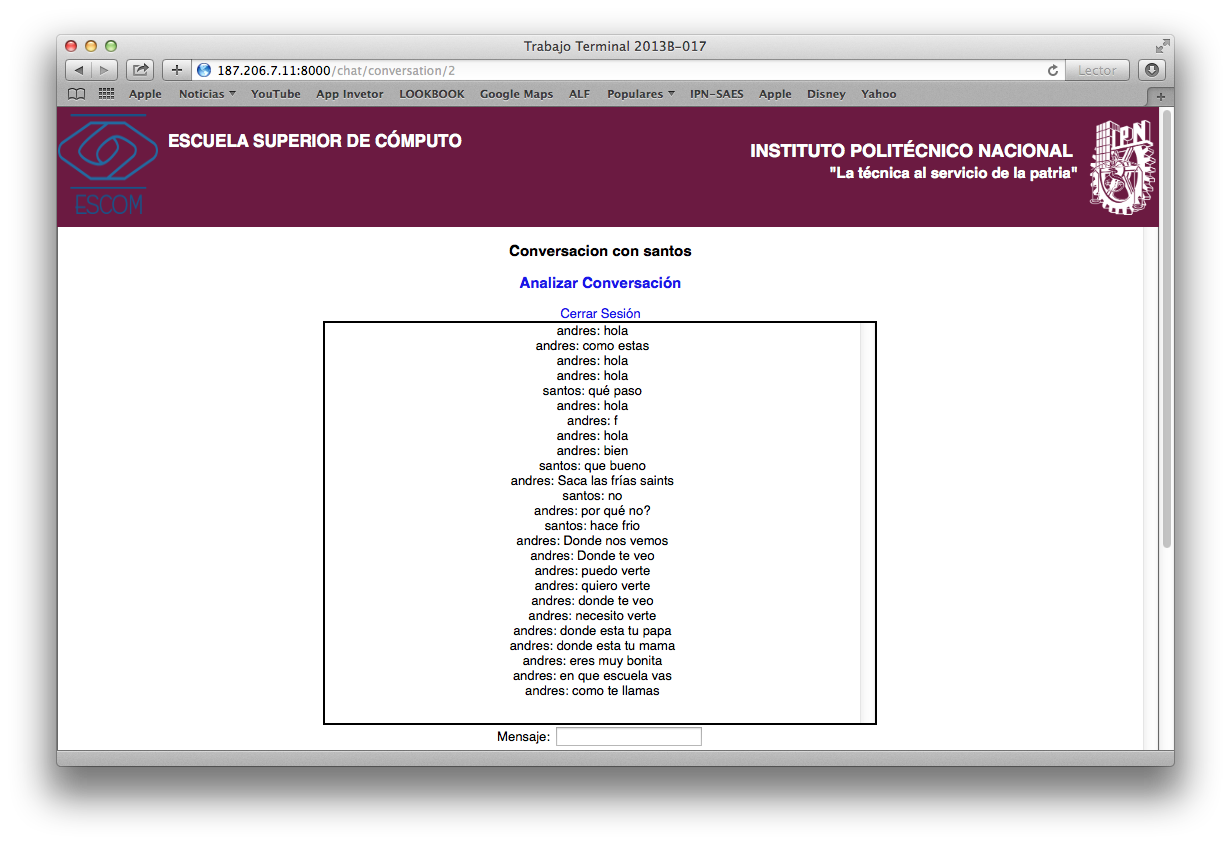
\includegraphics[width=0.9\textwidth]{images/Modulo1/Chat}
		\caption{Pantalla del sistema de mensajer\'ia}
	\end{figure}

\subsubsection{Salidas}
Conversaci\'on


\subsubsection{Entradas}
\begin{Citemize}

\item Mensaje 

\end{Citemize}
\subsubsection{Comandos}
\begin{itemize}
	\item \IUbutton{Enviar Mensaje}: Se env\'ia la cadena de caracteres contenida en el campo "Mensaje" a otro usuario del sistema. 
	\item \IUbutton{Analizar Conversaci\'on}: Muestra el an\'alisis de la conversaci\'on actualmente mostrada.
		\item \IUbutton{Cerrar sesi\'on}: Termina la sesi\'on y regresa a la p\'agina de inicio.
	\end{itemize}

\subsubsection{Mensajes}
Ninguno




	\pagebreak%%%%%%%%%%%%%%%%%%%%%%%%%%%%%%%%%%%%%%%%%%%%%%%%%%

	
	
	
	
			\subsection{IU5 Pantalla del An\'alisis (Gr\'afica)}

\subsubsection{Objetivo}
	El objetivo de esta pantalla es que el usuario pueda visualizar los resultados del an\'alisis realizado a la conversaci\'on solicitado.

\subsubsection{Dise\~no}
	Esta pantalla aparece despu\'es de solicitar el an\'alisis de la conversaci\'on en la pantalla del chat.

	\begin{figure}[htbp!]
		\centering
			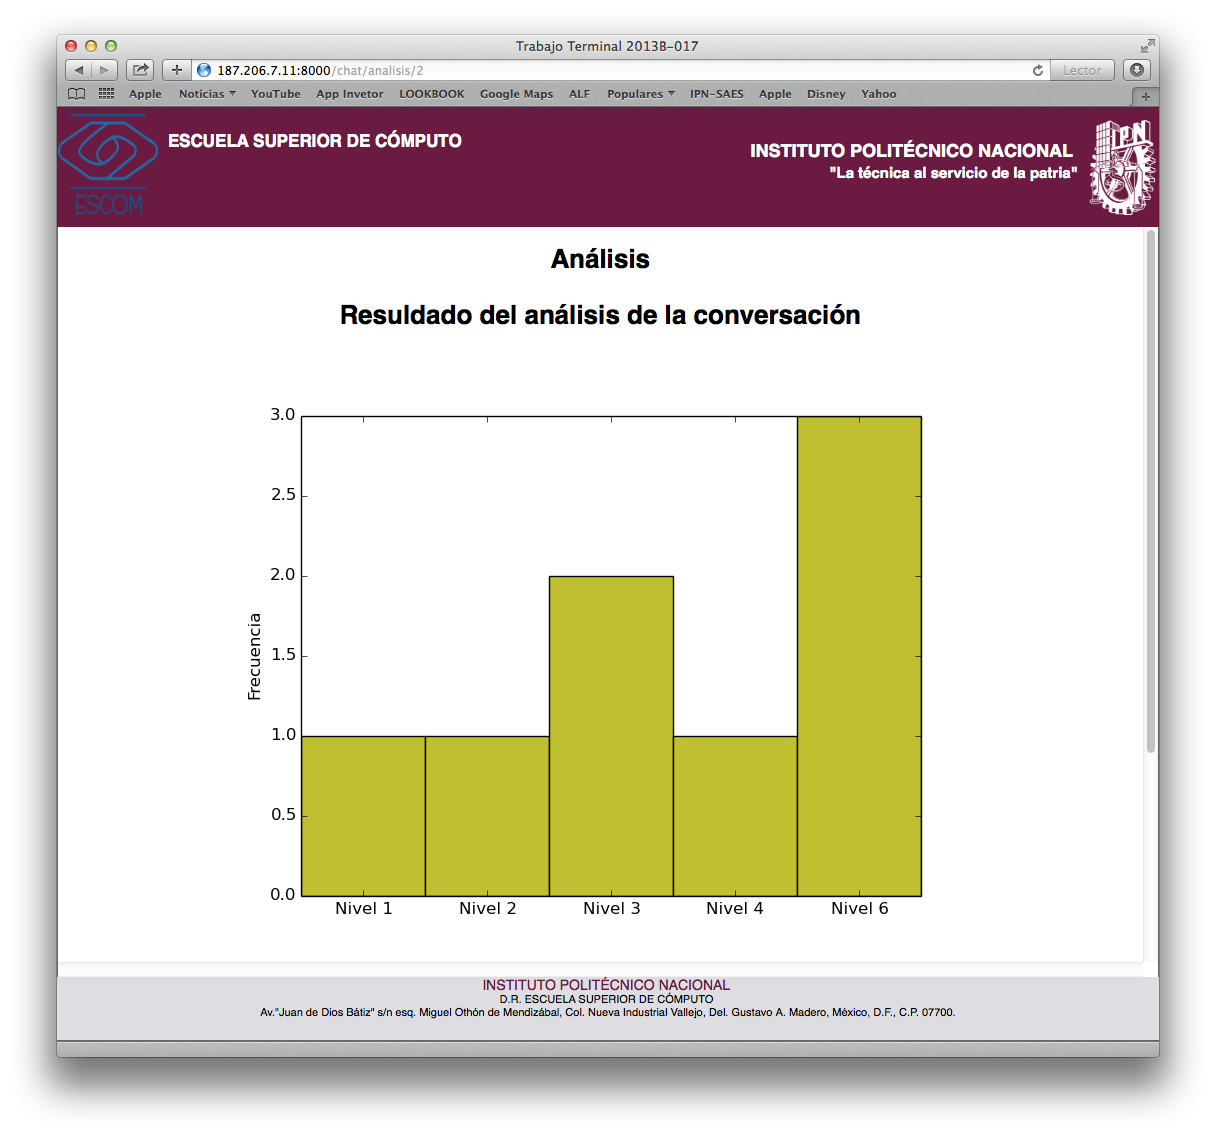
\includegraphics[width=0.9\textwidth]{images/Modulo1/GraficaAnalisis}
		\caption{Pantalla del An\'alisis (Gr\'afica)}
	\end{figure}

\subsubsection{Salidas}
Ninguna


\subsubsection{Entradas}
Ninguna
\subsubsection{Comandos}
Ninguno
\subsubsection{Mensajes}
Resultados del an\'alisis de la conversaci\'on 

\begin{figure}[htbp!]
		\centering
			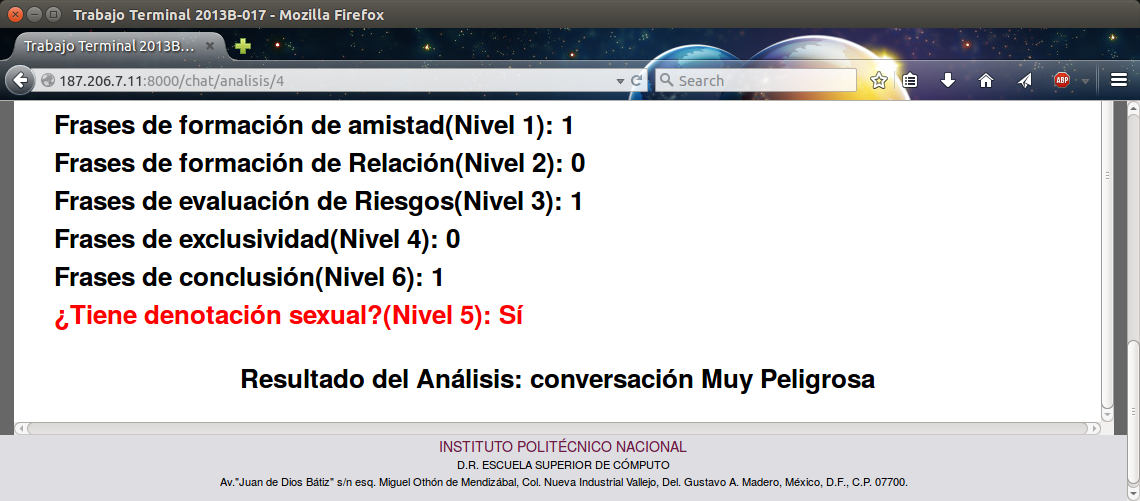
\includegraphics[width=0.9\textwidth]{images/Modulo1/InsidenciasNivel}
		\caption{Pantalla del An\'alisis (Incidencias)}
	\end{figure}



	\pagebreak%%%%%%%%%%%%%%%%%%%%%%%%%%%%%%%%%%%%%%%%%%%%%%%%%%

